\section{Menu Phase: 2D Renderer}
With the VGA up and running and a robust triple buffering system ready to operate, the game finally starts. The player enters the 2D renderer which displays menus to setup the 3D game. This is pretty simple yet features a nice VGA trick to turn the four banks' weak and cumbersome design into a strength.
\par
\begin{figure}[H]
\centering
\fullimage{first_menu.png}
\end{figure}
\par

Notice how the background of the menu screen is full red. This is a lot of pixels to write (320x200=64,000). With control over the bank mask, it is possible to write up to four pixels to the VRAM with only one write operation to the RAM. In the following VGA layout, you can see how pixels 0, 1, 2, and 3 are in different banks but at the same address (0x0000). By configuring the bank mask to 8+4+2+1 (15), it is possible to write to all banks simultaneously (e.g. write to 0x0000 writes pixels 0,1,2, and 3).\\
\par
\begin{figure}[H]
\centering
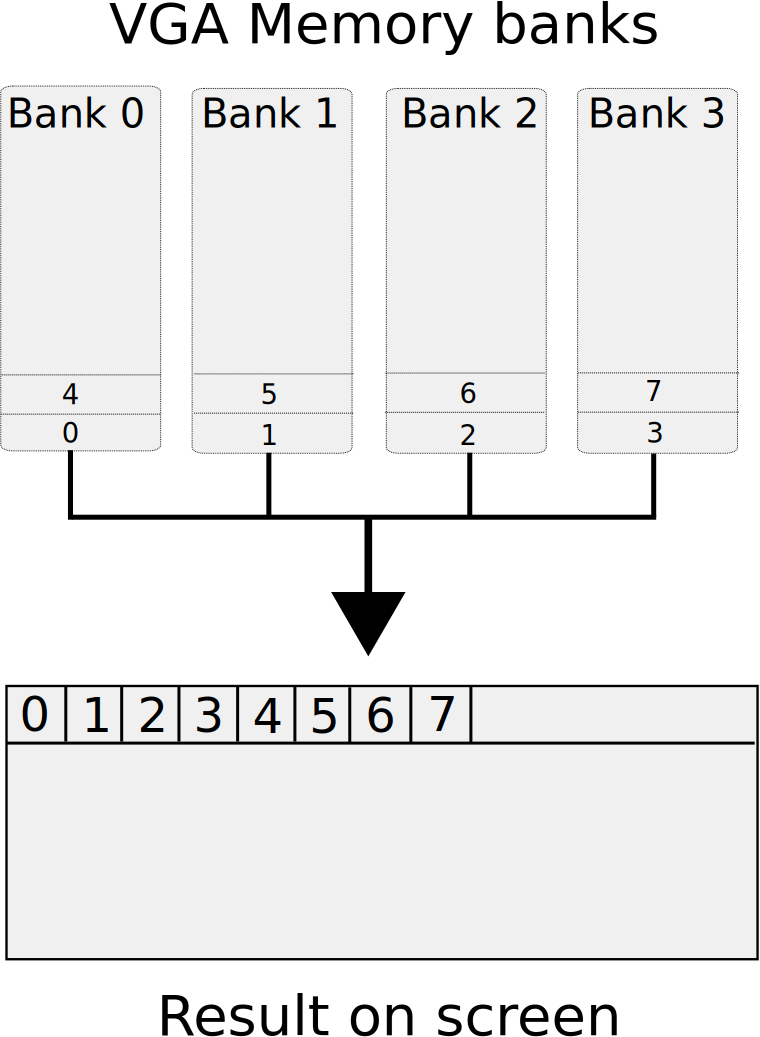
\includegraphics[width=0.6\textwidth]{imgs/drawings/vga_ram_screen_layout.pdf}
\caption{How bytes are read from the VRAM banks and displayed onto the screen.}
\end{figure}

\par
In order to clear the screen to red before drawing the menu, the 2D engine only performs 320x200/4 = 16,000 writes instead of 64000. In the drawing above, pixels 0,1,2, and 3 are written with one write operation. Then pixels 4,5,6, and 7 with another write, and so on and so forth.\\
\par
Even better, since the RAM can be written with 16 bit register, 8 pixels can be written in one RAM operation. A full screen can be cleared with 320x200/8 = 8,000 writes.
\par
\begin{minipage}{\textwidth}
\lstinputlisting[language=C]{code/vga_clear/optimal.c}
\end{minipage}
However, there is a limitation to this trick: only bytes at the same address in a bank can be written simultaneously. Pixel alignment with banks has to be carefully considered.\
\par
\begin{figure}[H]
\centering
 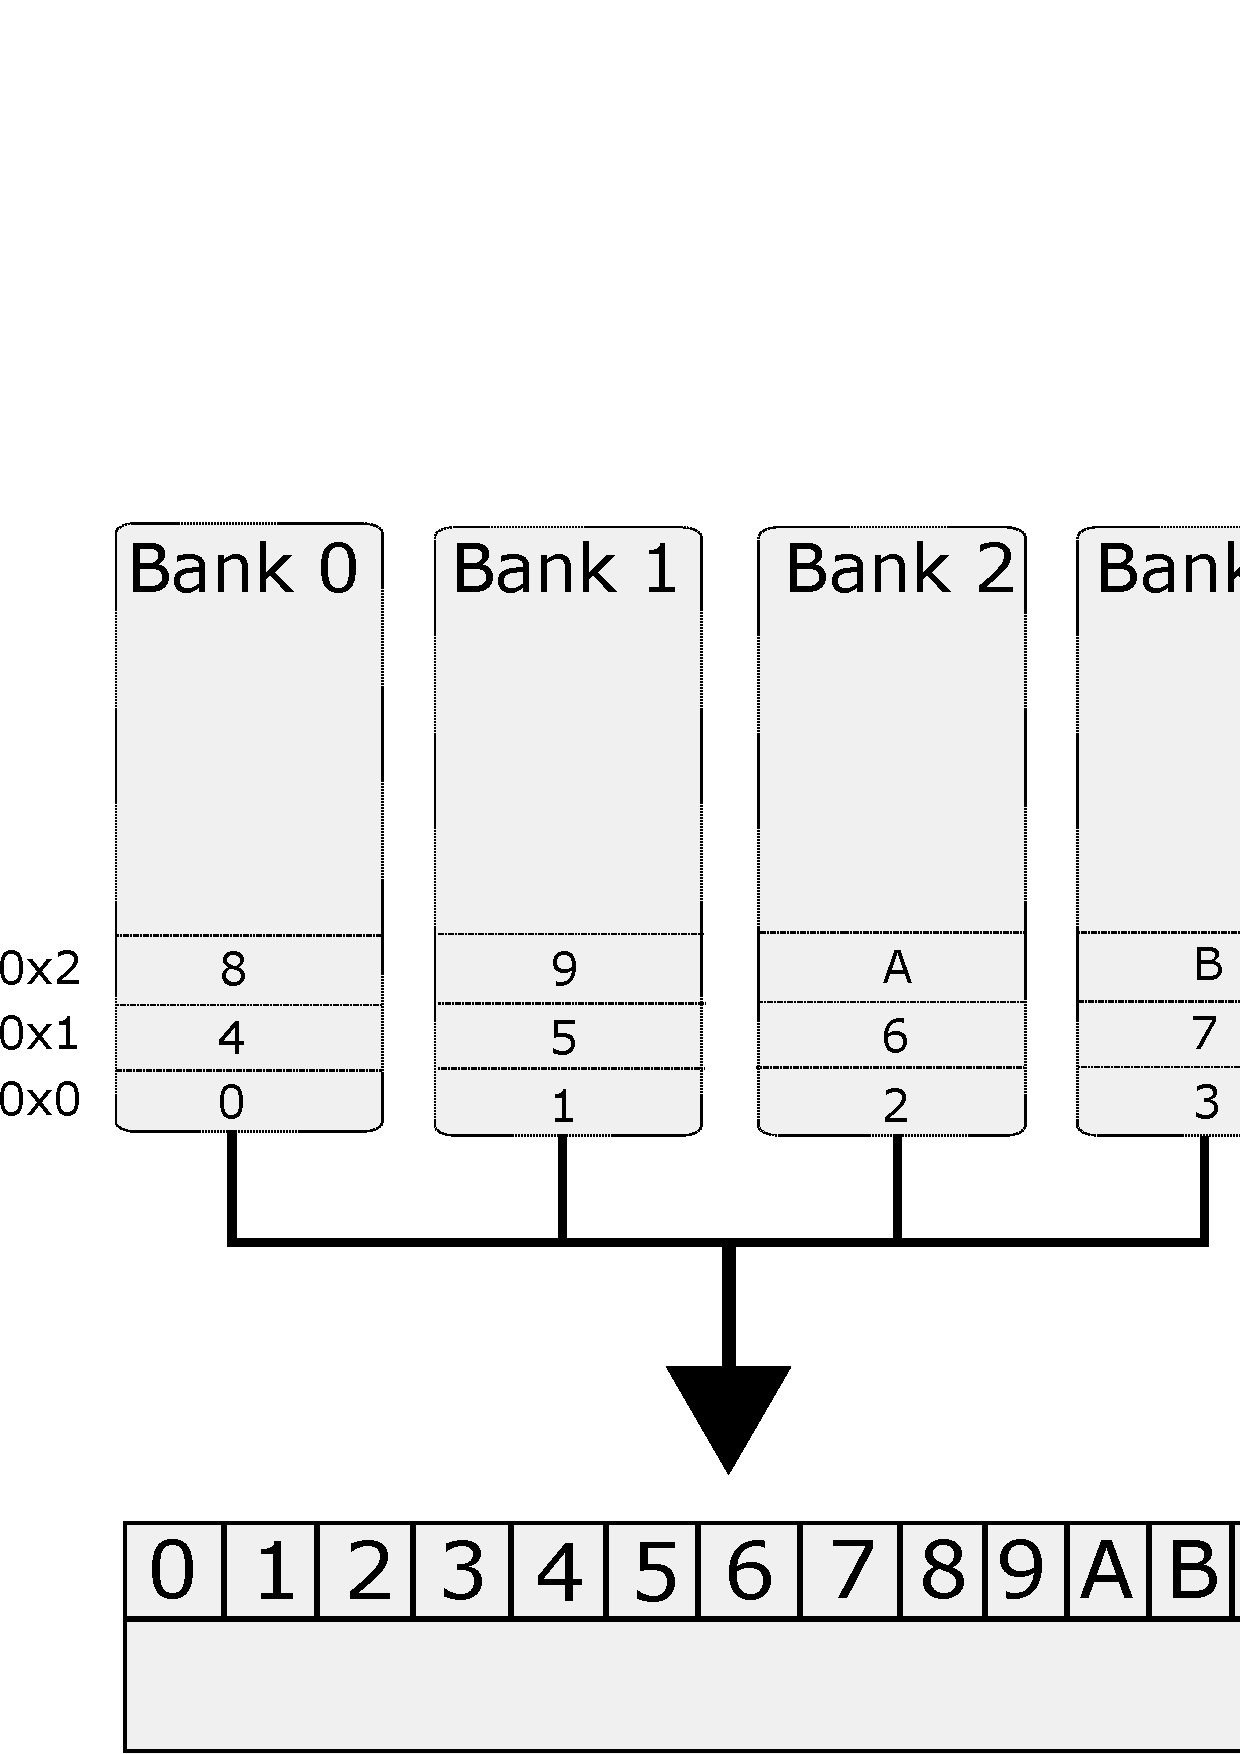
\includegraphics[width=.7\textwidth]{imgs/drawings/scalePost_explanation1.pdf}
 
 \end{figure}
Pixels 0, 1, 2, 3 can be written in one write.\\
Pixels 3 and 4 need two writes.\\
Pixels 3, 4, 5, 6, 7, 8 need three writes\footnote{How the mask allows for writing multiple pixels at once is extensively described on page \pageref{simd_vga}.}.\\


\par
The rest of the 2D renderer is pretty straight forward. It uses the User Manager extensively to render text and the Cache Manager to retrieve assets from HDD to RAM. Note that assets are called "pic" as opposed to "sprites" in the 3D renderer. Pictures are all Huffman-compressed (VGADICT, VGAHEAD, VGAGRAPH). Menus are stored in an array of struct. Here is the code to draw the "Main Menu" shown previously.\\

\par
\begin{minipage}{\textwidth}
\lstinputlisting[language=C]{code/menu.c}
\end{minipage}

\par
\begin{minipage}{\textwidth}
\lstinputlisting[language=C]{code/draw_main_menu.c}
\end{minipage}
\par
Notice how the \cw{C\_*} are macro defined in the files generated by \cw{IGRAB-ed}, the assets compiler.

